\documentclass[border=12pt]{standalone}
\usepackage[T1]{fontenc}
\usepackage[utf8]{inputenc}
\usepackage{lmodern}
\usepackage{tikz}
\usetikzlibrary{shapes.geometric, arrows.meta, positioning, calc, fit, backgrounds}

\begin{document}
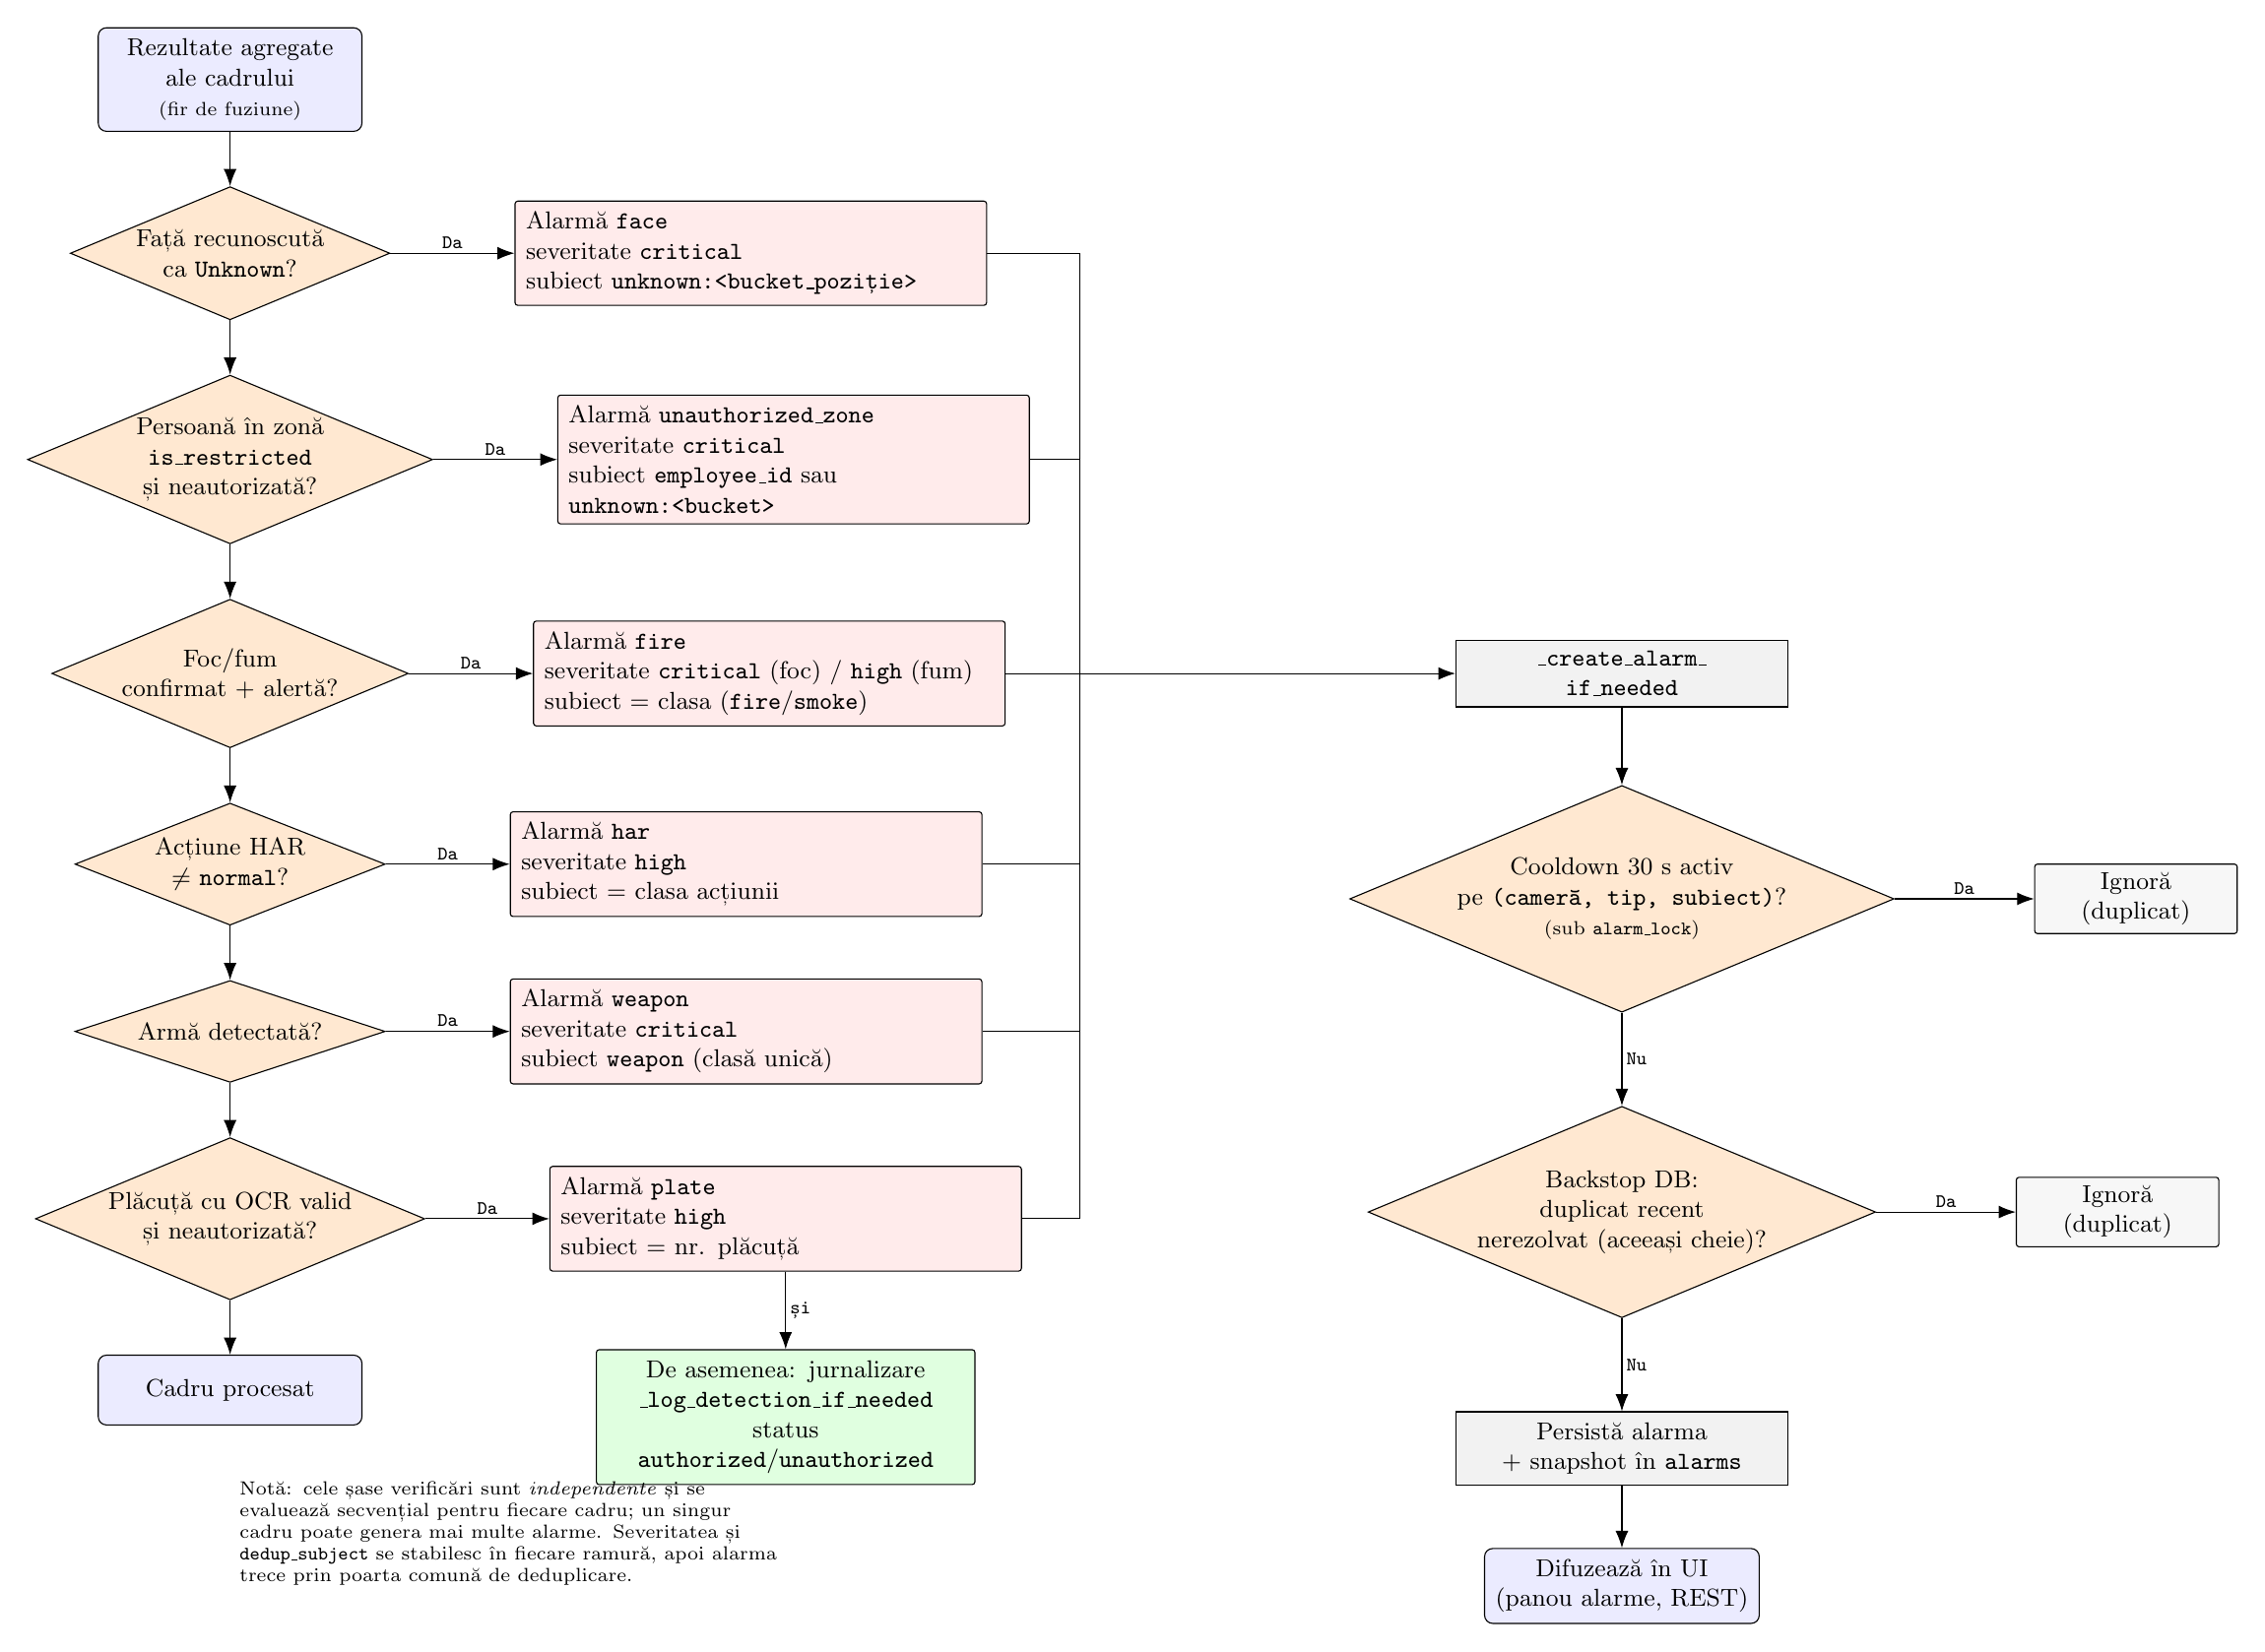
\begin{tikzpicture}[
  font=\small,
  >={Latex[length=2.2mm]},
  node distance=7mm and 16mm,
  io/.style   ={rounded corners=3pt, draw, fill=blue!8,  align=center, inner sep=4pt, minimum height=9mm, minimum width=34mm},
  dec/.style  ={diamond, aspect=2.4, draw, fill=orange!18, align=center, inner sep=1pt, minimum width=40mm},
  alarm/.style={draw, fill=red!8, align=left, inner sep=4pt, text width=58mm, rounded corners=1pt},
  proc/.style ={draw, fill=gray!10, align=center, inner sep=4pt, minimum height=8mm, text width=40mm},
  logn/.style ={draw, fill=green!12, align=center, inner sep=4pt, text width=46mm, rounded corners=1pt},
  ign/.style  ={draw, fill=gray!6, align=center, inner sep=3pt, minimum height=7mm, text width=24mm, rounded corners=1pt},
  lbl/.style  ={font=\scriptsize\ttfamily, inner sep=1.5pt},
  cd/.style   ={font=\ttfamily},
]

% ---------- left spine: input + six sequential checks ----------
\node[io] (in) {Rezultate agregate\\ale cadrului\\{\scriptsize(fir de fuziune)}};
\node[dec, below=of in]  (d1) {Față recunoscută\\ca {\ttfamily Unknown}?};
\node[dec, below=of d1]  (d2) {Persoană în zonă\\{\ttfamily is\_restricted}\\și neautorizată?};
\node[dec, below=of d2]  (d3) {Foc/fum\\confirmat + alertă?};
\node[dec, below=of d3]  (d4) {Acțiune HAR\\$\neq$ {\ttfamily normal}?};
\node[dec, below=of d4]  (d5) {Armă detectată?};
\node[dec, below=of d5]  (d6) {Plăcuță cu OCR valid\\și neautorizată?};
\node[io, below=of d6]   (end) {Cadru procesat};

% ---------- middle column: alarm payloads ----------
\node[alarm, right=of d1] (b1) {Alarmă {\ttfamily face}\\severitate {\ttfamily critical}\\subiect {\ttfamily unknown:<bucket\_poziție>}};
\node[alarm, right=of d2] (b2) {Alarmă {\ttfamily unauthorized\_zone}\\severitate {\ttfamily critical}\\subiect {\ttfamily employee\_id} sau {\ttfamily unknown:<bucket>}};
\node[alarm, right=of d3] (b3) {Alarmă {\ttfamily fire}\\severitate {\ttfamily critical} (foc) / {\ttfamily high} (fum)\\subiect = clasa ({\ttfamily fire}/{\ttfamily smoke})};
\node[alarm, right=of d4] (b4) {Alarmă {\ttfamily har}\\severitate {\ttfamily high}\\subiect = clasa acțiunii};
\node[alarm, right=of d5] (b5) {Alarmă {\ttfamily weapon}\\severitate {\ttfamily critical}\\subiect {\ttfamily weapon} (clasă unică)};
\node[alarm, right=of d6] (b6) {Alarmă {\ttfamily plate}\\severitate {\ttfamily high}\\subiect = nr. plăcuță};

% spine arrows (checks run sequentially & independently for every frame)
\draw[->] (in) -- (d1);
\draw[->] (d1) -- (d2);
\draw[->] (d2) -- (d3);
\draw[->] (d3) -- (d4);
\draw[->] (d4) -- (d5);
\draw[->] (d5) -- (d6);
\draw[->] (d6) -- (end);

% "Da" side branches to alarm payloads
\foreach \d/\b in {d1/b1,d2/b2,d3/b3,d4/b4,d5/b5,d6/b6}
  \draw[->] (\d) -- node[lbl,above]{Da} (\b);

% ---------- collector bus on the right of the alarm boxes ----------
\coordinate (busx) at ($(b1.east)+(12mm,0)$);
\node[proc, right=58mm of b3] (tail0) {\ttfamily \_create\_alarm\_\\if\_needed};
% route every alarm box into a single vertical bus, then one feed to the tail
\foreach \b in {b1,b2,b3,b4,b5,b6}
  \draw (\b.east) -- (busx |- \b);
\draw (busx |- b1) -- (busx |- b6);
\draw[->] (busx |- tail0) -- (tail0.west);

% ---------- common tail: dedup + cooldown + DB backstop + persist ----------
\node[dec, below=10mm of tail0] (cool) {Cooldown 30~s activ\\pe {\ttfamily (cameră, tip, subiect)}?\\{\scriptsize(sub {\ttfamily alarm\_lock})}};
\node[ign, right=18mm of cool]  (ign1) {Ignoră\\(duplicat)};
\node[dec, below=12mm of cool]  (db)   {Backstop DB:\\duplicat recent\\nerezolvat (aceeași cheie)?};
\node[ign, right=18mm of db]    (ign2) {Ignoră\\(duplicat)};
\node[proc, below=12mm of db]   (persist) {Persistă alarma\\+ snapshot în {\ttfamily alarms}};
\node[io, below=8mm of persist] (broadcast) {Difuzează în UI\\(panou alarme, REST)};

\draw[->] (tail0) -- (cool);
\draw[->] (cool)  -- node[lbl,above]{Da} (ign1);
\draw[->] (cool)  -- node[lbl,right]{Nu} (db);
\draw[->] (db)    -- node[lbl,above]{Da} (ign2);
\draw[->] (db)    -- node[lbl,right]{Nu} (persist);
\draw[->] (persist) -- (broadcast);

% ---------- plate also gets logged (alarm AND log) ----------
\node[logn, below=10mm of b6] (log) {De asemenea: jurnalizare\\{\ttfamily \_log\_detection\_if\_needed}\\status {\ttfamily authorized}/{\ttfamily unauthorized}};
\draw[->] (b6.south) -- node[lbl,right]{și} (log.north);

% ---------- legend note ----------
\node[align=left, font=\scriptsize, text width=70mm, below=6mm of end, anchor=north west] (note)
  {Notă: cele șase verificări sunt \emph{independente} și se evaluează secvențial pentru fiecare cadru; un singur cadru poate genera mai multe alarme. Severitatea și {\ttfamily dedup\_subject} se stabilesc în fiecare ramură, apoi alarma trece prin poarta comună de deduplicare.};

\end{tikzpicture}
\end{document}
